\chapter{Урамшууллын систем}
\section{Төслийн зорилго}
Hoome аппликейшнд шинэ хэрэглэгчдийг татах, нийт хэрэглэгч дунд аппликейшны
хэрэглээг өргөжүүлэх, улмаар Hoome аппликейшны зах зээлд өрсөлдөх чадварыг
нэмэгдүүлэх зорилгоор тус аппликейшн дээр оноо цуглуулах системийг хэрэгжүүлж
байна. Хэрэглэгчид оноо (цаашид HPoint гэж нэрлэнэ) цуглуулж түүгээрээ олон төрлийн
хөнгөлөлт, урамшууллыг эдлэх боломжийг нээнэ. Цаашлаад Hoome аппликейшныг
цахим мөнгөний хэтэвчтэй болгох эхлэлийг тавихад энэ төслийн зорилго оршино.

\section{Хамрах хүрээ}
Энэхүү төслийн хэтийн зорилго нь цахим мөнгөний хэтэвчтэй болох, түүний хэрэглээг
өдөр тутмын амьдралд оруулах юм. Цахим хэтэвч гэдэг нь Монгол улсын төлбөрийн
үндсэн хэрэгсэлт “төгрөг” болон түүнтэй дүйцэхүйц солилцоог хийх боломжой байх
ёстой.
Энэхүү үндсэн зорилго хүртэл дараах үе шатууд хэрэгжинэ:

\begin{enumerate}
  \item Урамшууллын оноо цуглуулах, зарцуулах боломжтой болох
  \begin{itemize}
    \item Цуглуулах - Дахин давтагдашгүй хэрэглэгчийн редим кодтой байх.
    Түүгээр уригдсан хүмүүсийн лимит, оноог тооцон цуглуулах
    \item Зарцуулах - Оноог төгрөгтэй дүйцүүлэн Hoome аппликейшнээр хийх
    боломжтой төлбөрт оролцуулах
  \end{itemize}
  \item Бусад дижитал бүтээгдэхүүн, платформд ашиглагддаг хэтэвчтэй интеграци хийх
  боломжтой болгох
  \begin{itemize}
    \item ITStore (cody) хэтэвчнээс үлдэгдэл төгрөгийг HPoint болгон хөрвүүлж
    оноо болгох
    \item HPoint оноог буцаагаад Itstore хэтэвч рүү хөрвүүлэх
  \end{itemize}
  \item Хэтэвчтэй бусад төрлийн дижитал бүтээгдэхүүнээ холбох, HPoint болгон
  цуглуулдаг болгох
\end{enumerate}

\begin{figure}[h]
\centering
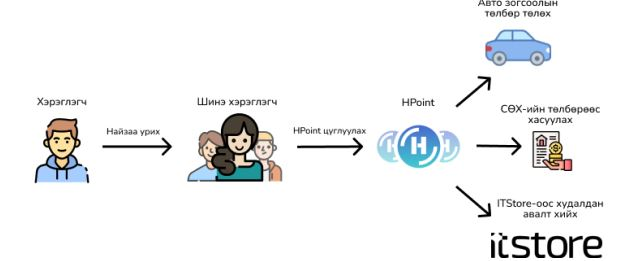
\includegraphics{imgs/hpointUseCase.JPG}
\end{figure}

\section{Шаардлага}
\begin{table}[h]
  \caption{HPoint ФШ}
  \begin{tabular}{|p{1cm}|p{6cm}|p{6cm}|l|}
    \hline
    ID & Шаардлага & Тайлбар & Төрөл \\ \hline
    ФШ01 & Хэрэглэгч шинэ хэрэглэгчдийг урих өөрийн гэсэн давтагдашгүй кодтой байна. & Тухайн кодоо бусдад өгөх замаар шинэ хэрэглэгчдийг урина. & Зайлшгүй \\ \hline
    ФШ02 & Хэрэглэгч аппликейшинд шинээр бүртгүүлэхдээ найзын урилгаа оруулах талбартай байна. & Уригдсан хэрэглэгч тухайн талбарт урилгын кодоо оруулна. & Зайлшгүй \\ \hline
    ФШ03 & Шинэ хэрэглэгч утасны дугаараа баталгаажуулсны дараа урилга баталгааждаг байна. &Ингэснээр хуурамч хэрэглэгч үүсэхээс сэргийлэхийн зэрэгцээ байгууллагаас гарах зарлагын тааз үнийг тооцоолох боломжтой болно. & Зайлшгүй \\ \hline
    ФШ04 & Хэрэглэгч бүр өөрийн гэсэн HPoint оноог цуглуулдаг хэтэвчтэй байна. & Хэрэглэгч тухайн оноогоо ашиглаж хөнгөлөлт, урамшуулал авахад тохирох дүнгээр хэтэвчийг нь шинэчилдэг байх. & Зайлшгүй \\ \hline
    ФШ05 & Хэрэглэгч цуглуулсан HPoint оноогоо ашиглан СӨХ-ийн төлбөрөөс хасуулах боломжтой байна. & Зөвхөн Hoome-д нэвтэрсэн СӨХ-тэй өрхүүдэд хүчинтэй & Зайлшгүй \\ \hline
  \end{tabular}
\end{table}

\begin{table}[h]
  \begin{tabular}{|p{1cm}|p{6cm}|p{6cm}|l|}
    \hline
    ФШ06 & Хэрэглэгч цуглуулсан HPoint оноогоо ашиглан зогсоолын төлбөр төлөх боломжтой байна. & Зөвхөн CCP ашигладаг зогсоолуудад хүчинтэй & Зайлшгүй \\ \hline
    ФШ07 & Хэрэглэгч урилгаар бүртгүүлэхэд түүнийг урисан болон урилга хүлээн авсан хэрэглэгч тус бүр 1000 HPoint авна. & Урисан ба уригдсан хүмүүст хоёуланд нь HPoint бэлэглэнэ. & Зайшлгүй \\ \hline
    ФШ08 & Нэг хэрэглэгч сард 5-аас илүүгүй шинэ хэрэглэгч урих хязгаартай байна. && Зайлшгүй \\ \hline
    ФШ09 & Хэрэглэгч ITStore дээр бүртгэлтэй бол ITStore-ын хэтэвч рүүгээ HPoint-оо оруулах, & ITStore-ын хэтэвчин дэх үлдэгдлээ Hoome аппликейшн рүү HPoint болгон хөрвүүлж болдог байна. Хоёр талын гүйлгээг дэмждэг байна & Зайлшгүй \\ \hline
  \end{tabular}
\end{table}
